\documentclass[tikz,border=5mm]{standalone}

\begin{document}

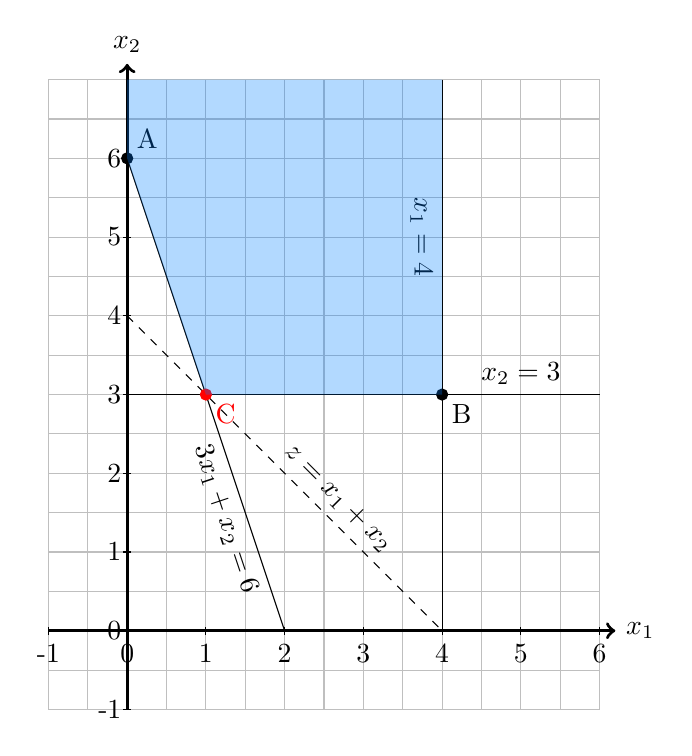
\begin{tikzpicture}

    \draw[gray!50, thin, step=0.5] (-1,-1) grid (6,7);
    \draw[very thick,->] (-1,0) -- (6.2,0) node[right] {$x_1$};
    \draw[very thick,->] (0,-1) -- (0,7.2) node[above] {$x_2$};

    \foreach \x in {-1,...,6} \draw (\x,0.05) -- (\x,-0.05) node[below] {\x};
    \foreach \y in {-1,...,6} \draw (-0.05,\y) -- (0.05,\y) node[left] {\y};

    \draw (0,3) -- (4,3) -- node[above] {$x_2=3$}  (6,3);
    \draw (4,7) -- node[below,sloped] {$x_1=4$} (4,3) -- (4,0);
    \draw (0,6) -- (1,3) -- node[below,sloped] {$3x_1+x_2=6$} (2,0);
    \draw[dashed] (0,4) -- (1,3) -- node[above, sloped] {$z=x_1+x_2$} (4,0);

    \filldraw [black] (0,6) circle (2pt) node[above right] {A};
    \filldraw [black] (4,3) circle (2pt) node[below right] {B};
    \filldraw [red] (1,3) circle (2pt) node[below right] {C};

    \fill[blue!50!cyan,opacity=0.3] (0,6) -- (0,7) -- (4,7) -- (4,3) -- (1,3) -- (0,6);

\end{tikzpicture}

\end{document}
